
% \newcommand {\matr}[2]{\left[\begin{array}{#1}#2\end{array}\right]}
% \newcommand{\E}{\mathbb{E}}
% \newcommand{\tr}{\mathrm{tr}}
% \newcommand{\x}{{\mathbf{x}}}
% % \renewcommand{\u}{{\mathbf{u}}}
% \newcommand{\w}{{\mathbf{w}}}
% \renewcommand{\r}{{\mathbf{r}}}

% \makeglossaries
% \sisetup{
% display-per-mode = fraction,
% inline-per-mode = symbol,
% group-separator = {,}
% }

% Acronym definitions
\glsresetall
\newacronym{mdp}{MDP}{Markov Decision Process}
\newacronym{pomdp}{POMDP}{Partially Observable Markov Decision Process}
\newacronym{lstm}{lstm}{long short-term memory}
\newacronym{dqn}{DQN}{deep Q-network}
\newacronym{idm}{IDM}{intelligent driver model}
\newacronym{rl}{RL}{reinforcement learning}
\newacronym{ad}{AD}{autonomous driving}
\newacronym{av}{AV}{autonomous vehicles}
\newacronym{adas}{ADAS}{advance driver assistance systems}

%%%%%%%%%%%%%%%%%%%%%%%%%%%%%%%%%%%%%%%%%%%%%%%%%%%%%%%%%%%%%%%%%%%%%%%%%%%%%%%%
\begin{abstract}
This paper investigates different approaches to find a safe and efficient driving strategy through an intersection with other drivers.
Because the intentions of the other drivers to yield, stop, or go are not observable, we use a particle filter to maintain a belief state. 
We study how a reinforcement learning agent can use these representations efficiently during training and evaluation.
This paper shows that an agent trained without any consideration of the intentions of others is both slower at reaching the goal and results in more collisions.
Four algorithms that use a belief state generated by a particle filter are compared. Two of the algorithms have access to the intention only during training while the others do not. The results show that explicitly trying to predict the intention gave the best performance in terms of safety and efficiency.

\end{abstract}

\section{Introduction}
\label{sec:introduction}

During the last decade, major progress has been made towards deploying \gls{av} and improving traffic safety. 
Structured traffic scenarios can often be solved by rule-based or planning-based methods, where the surrounding vehicles are assumed to follow a simple driving model. However, according to the Insurance Institute for Highway Safety~\cite{IIHS2019}, in 2019, an estimated \num{115741} people were injured by drivers running a red light and \num{928} of them were killed. 
Hence, to give \gls{av} the capability to avoid accidents when other traffic participants do not follow the rules, they need the capability to consider the intentions and predict future actions of other participants. 
% It is therefore not enough to only rely on the traffic signs and lights but also necessary for \gls{av} to be able to also consider the intentions and predict the future actions of other traffic participants. 
For example, in an intersection or a roundabout scenario, a human driver would observe other vehicles and form a belief of the driver's intention to yield or not and would then act according to this belief. Although \gls{av}s have the potential to simultaneously observe more objects than a human, there is a vast number of possible traffic situations, making it difficult for an engineer to anticipate every situation and design a suitable rule-based strategy. Furthermore, both traffic rules and driving styles vary between different countries. Therefore, we focus on approaches that instead learn from experience how to behave in different situations and adapt to different driving styles. A desirable property of such a learning-based agent is that it accounts for the intentions of the surrounding traffic participants.

Using \gls{rl} to create a general decision-making agent for autonomous driving has been suggested in many studies during the last few years. For example, \citet{Isele2018} demonstrated how the \gls{dqn} algorithm could be used to navigate through occluded intersections. \Citet{chen2019} compared the performance of \gls{dqn} with policy gradient and an actor critic method for different roundabout scenarios. 
An overview of RL-based studies for autonomous driving is given by \citet{Ye2021} and \citet{kiran2021}.
Most of these studies both train and evaluate the agents in simulated environments, whereas \citet{Bansal2018} and \citet{Pan2017} focus on transferring an agent that has been trained in simulation to drive in the real world. \Citet{Kendall2019} trained in the real world.
Game-theoretic approaches to unsignalized intersection scenarios have been proposed by \citet{chen2020} and \citet{li2021}. A drawback is that these methods are limited by their models of other driver intentions and the prediction of their future actions. Therefore, we propose using \gls{rl} to learn a policy based on experience. 
% However, a drawback is that these methods do not explicitly consider the intentions of the drivers of the surrounding vehicles. 


The decision-making task of an autonomous vehicle can be formulated as a \gls{pomdp}, e.g., where the intentions of other traffic participants are included in the state space but are not directly observable. 
\Citet{Sunberg2017} models freeway lane changes as a \gls{pomdp} with latent internal states and found a policy using Monte Carlo Tree Search. 
Our previous work~\cite{Tram2018} showed that it was possible for an agent to solve such a \gls{pomdp} by finding gaps between cars in an intersection by using a \gls{lstm}, but the intentions were not explicitly estimated. In this paper, we hypothesize that explicitly estimating the intention probability distribution of the other drivers can improve the performance of the policy by reducing the number of collisions and reach the other side of the intersection faster. \Citet{Hubmann2017} proposed a similar \gls{pomdp} framework for solving the same intersection problem using a particle filter, but they did not use \gls{rl}. By using \gls{rl}, the method is more scalable to different environments and has the potential to adapt to real world behaviors through experience. 

This hypothesis, that explicitly estimating the intention can reduce the number of collisions, is verified by training and comparing two \gls{dqn} agents: one with full observability (\textbf{DQN FO}) including the true intention as an input feature to the network; and one without intention, that is referred to as \textbf{DQN without intention}. While we show in our simulations that observing the true intention leads to performance improvements, it is not a realizable approach in practice since the intention is not observable. 
We will therefore investigate and answer the following questions: \textit{How can the intention of the other vehicles approaching an intersection be estimated?} 
\textit{With a belief state, is it better to train on the full distribution of the belief or use an estimate of the intention?} \textit{Can the approximation of the neural network compensate for the inaccuracy of the particle filter?}

To answer the first question, a particle filter is proposed in \ref{sec:particle_filter}, which uses a sequence of past observations to generate a belief state. This belief state can then be used, instead of the true intent, to create a policy. 
In addition to the two baseline DQN agents, four approaches that combine a particle filter with the \gls{dqn} algorithm are presented in \ref{sec:belief_state_rl}. The \textbf{Q Particle Filter (QPF)} approach uses the belief state, i.e., the full set of particles to estimate the $Q$-values both during the training and evaluation processes. 
If the intention is accessible during training the second approach, \textbf{QMDP}, is trained under full observability and then tested with the belief state as input. The third approach, \textbf{Q Intention Distribution (QID)}, only uses a probability distribution of the non-observable states as an input both during the training and testing processes. Finally, \textbf{QMDP-Intention Estimate (QMDP-IE)} is trained under full observability and tested with an estimate of the intention from the particle filter. The detail of each approach are explained in more detail in \ref{sec:belief_state_rl} and their performance is evaluated in an unsignalized intersection scenario, explained in \ref{sec:experiments}.


The results show that the intention state improves the policy when comparing the performance between a \gls{dqn} with access to the true intention and a \gls{dqn} without the intention state. The QMDP-IE algorithm found the safest policy with zero collisions in the evaluation set, while the QID found the fastest and most aggressive policy.

The main contributions of this paper are: 
\begin{itemize}
    \item Multiple \gls{dqn} models that capture the belief state at training time either in the form of particle, point estimate of the intention, or the likelihood of the intention.
    \item A particle filter approach for estimating the intentions of surrounding traffic participants in an intersection.
    \item Empirical analysis of the performance of four approaches to explicitly consider the intentions of other traffic participants in an \gls{rl} framework.

\end{itemize}


The structure of the paper is as follows. In \ref{sec:background}, we review \gls{pomdp}s and the \gls{idm}. In \ref{sec:approach}, we formulate the problem as a \gls{pomdp} and introduce the particle filter used to generate the belief state along with the algorithms used to solve the \gls{pomdp}. In \ref{sec:experiments}, we describe the simulation setup, the neural network architecture, and training procedure. \ref{sec:results} compares the different algorithms and our conclusions are presented in \ref{sec:conclusion}. 

% \hfill mds
% \hfill August 26, 2020



\section{Background}
\label{sec:background}
This section briefly describes the \gls{pomdp} framework, the approximation method QMDP, deep Q-learning, and the \gls{idm}.  


\subsection{Partially observable Markov decision process}
A \gls{pomdp} is a mathematical framework used for modeling sequential decision making problems under uncertainty. 
It consists of a set of states $\mathcal{S}$, actions $\mathcal{A}$, observations $\Omega$, a transition model $T$, observation model $O$, reward function $R$, and a discount factor $\gamma$. 
Together they create the tuple $(\mathcal{S},\mathcal{A},\Omega,T,O,R,\gamma)$ that formally defines a \gls{pomdp}~\cite{Kochenderfer2015}. 
While in a state $s \in \mathcal{S}$ and executing an action $a \in \mathcal{A}$ the probability of transitioning to a future state $s^\prime$ is described by the transition model $T(s^\prime \mid s,a)$ and the reward $r$ is given by the reward function $R(s,a)$. 
The agent only has access to partial information contained in its observation $o$ distributed according to $\Pr(o \mid s', a) = O(o, s', a)$.

To accommodate for the missing information, the agent maintains a belief state. A belief state $b$ is a probability distribution such that $b(s) = \Pr(s \mid o_{1:t})$ is the probability of being in state $s$ given observations $o_{1:t}$. 
At each time step $t$, the agent updates its belief using a Bayesian filtering approach given the previous belief and the current observation as follows:
\begin{equation}
    b^\prime(s^\prime) \propto O(o \mid s^\prime, a) \sum_{s \in S}T(s^\prime \mid s,a)b(s).
\end{equation}

In a \gls{pomdp}, a policy is a mapping from a belief state to an action. A value function $Q^\pi(b, a)$ represents the expected discounted accumulated reward received by following policy $\pi$ after taking action $a$ from belief state $b$.
The goal is to find a policy, that maximizes the expected reward.
Finding such a policy is generally intractable~\cite{Kochenderfer2015}. We can use an approximation referred to as QMDP:

\begin{equation}
    Q(b, a) \approx \sum_s b(s) Q_{\mathrm{MDP}}(s, a)
    \label{eq:qmdp}
\end{equation}
where $Q_{\mathrm{MDP}}$ is the optimal value function of the \gls{mdp} version of the problem that assumes that the agent has full observability. 

While finding the optimal $Q(b, a)$ is intractable, finding $Q_{\mathrm{MDP}}$ is usually easier. 
When the transition function can be written explicitly and the state space is finite, we can use dynamic programming to compute $Q_{\mathrm{MDP}}$. 
Often, the transition function is only accessible in the form of a generative model (\textit{e.g.} a simulator) and the state space is high dimensional and continuous. 
In such settings, we can use deep Q-learning to approximate $Q_{\mathrm{MDP}}$~\cite{LITTMAN1995}. 

In deep Q-learning, the value function is approximated by a neural network. The function approximating the optimal value function is given by minimizing the following loss function:
\begin{equation}
    J(\theta) = E_{s^\prime}[(r + \gamma \max_{a^\prime}Q(s^\prime, a^\prime; \theta) - Q(s, a; \theta))^2]
    \label{eq:dqn-loss}
\end{equation}
where $\theta$ represents the weights of the neural networks and $(s, a, r, s')$ is obtained from one simulation step in the environment. 
The weights are updating through gradient updates. 
In addition, innovations such as the use of a replay buffer and a target network can greatly help the convergence~\cite{Mnih2015}. 

\subsection{Driver model}
\label{sec:driver_model}
The general behaviour of cars are modeled using \gls{idm}~\cite{idm2000} and the acceleration is described by
\begin{align*}
    & \alpha = \alpha_{\mathrm{max}}\Big(1-\Big(\frac{v_\alpha}{v_0}\Big)^\delta-\Big( \frac{s^*(v_\alpha,\Delta v_\alpha)}{s_\alpha}\Big)^2\Big) \\
    & \mathrm{with ~} s^*(v_\alpha, \Delta v_\alpha) = s_0 + v_\alpha T_{\mathrm{gap}} + \frac{v_\alpha \Delta v_\alpha}{2 \sqrt{a_{\mathrm{max}} \alpha_b}}
\end{align*}
where $v_0$ is the desired velocity, $s_0$ is the minimum distance between cars, $T_{\mathrm{gap}}$ is the desired time gap with the vehicle in front, $a_\mathrm{max}$ is the maximum vehicle acceleration, and $\alpha_b$ and $\delta$ are comfort braking deceleration and a model parameter. The velocity difference $\Delta v_\alpha$ between the two vehicles and the distance to the vehicle in front $s_\alpha$ determine the acceleration for the next time step. 
The acceleration can be simplified into two terms, one for free road with no lead vehicle
\begin{equation}
    a^\text{free}= \alpha_\mathrm{max}\Big(1-\Big(\frac{v_\alpha}{v_0}\Big)^\delta\Big)
    \label{eq:idm_free}
\end{equation}
and an interaction term for when there is a vehicle in front 
\begin{align}
     a^\text{int} &=  -a \Big(\frac{(s_\alpha,\Delta v_\alpha)}{s_\alpha} \Big) ^2 \\
     &= -a \Big(\frac{s_0 + v_\alpha T_{\mathrm{gap}}}{s_\alpha} + \frac{v_\alpha \Delta v_\alpha}{2 \sqrt{a_{\mathrm{max}} \alpha_b} s_\alpha} \Big) ^2.
     \label{eq:idm_int}
\end{align}
These equations are used to both model behaviors of other drivers and generate the acceleration for the ego vehicle.

\section{Proposed approach}
\label{sec:approach}

In this section, we define the main problem that this paper addresses, as well as its components. Further, the particle filter used to estimate the belief state is introduced. Finally, we present the RL algorithms that are used to train the agents.


\subsection{Problem formulation}
\label{sec:pomdp}

The problem setting is a four-way intersection shown in \ref{fig:states}. The ego vehicle approaches an intersection with at least one other car on the perpendicular lane with about the same time to intersection assuming a constant velocity model. The goal for the ego vehicle is to reach the other side of the intersection as fast as possible without colliding with the other car. With only onboard sensors on the ego vehicle, it can observe the physical state of other vehicles but not their intention. 
Such an intersection can be described as a \gls{pomdp}.

\subsubsection{State space, $\mathcal{S}$}
\begin{figure}[!t]
    \centering
        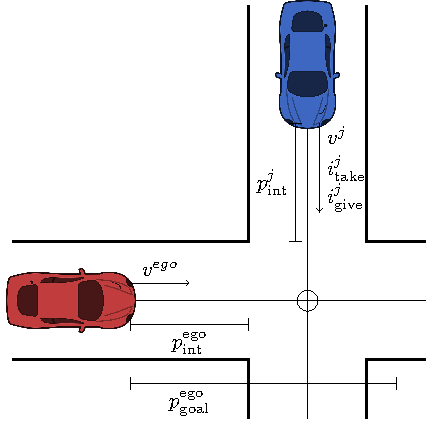
\includegraphics[width=0.6\columnwidth]{figures/figures-observations.pdf}
        \caption{State definitions for the intersection. The red vehicle is the ego vehicle.}
    \label{fig:states}
\end{figure}

The state of the system,
\begin{align}
    s = (p^\mathrm{ego}_\mathrm{goal},p^\mathrm{ego}_\mathrm{int}, v^\mathrm{ego}, t_\mathrm{stop}, \{p^{j}_\mathrm{int}, v^j, i^j\}_{j=1}^N),
    \label{eq:state}
\end{align}
consists of the ego vehicle state and the states of the surrounding vehicles. The ego vehicle state is described by the distance to the intersection $p^\mathrm{ego}_\mathrm{int}$, the distance to the goal $p^\mathrm{ego}_\mathrm{goal}$, and the velocity $v^\mathrm{ego}$. Stop time $t_\mathrm{stop}$ is the time the ego vehicle is at stand still $v^\mathrm{ego}=0$. This state tracks the amount of time the ego vehicle has been standing still at the intersection and indicates the time to the terminal states \textit{safe stop} or \textit{deadlock}, which are explained later when we define the reward function. The states of the surrounding vehicles, indexed by $j \in \{1, \ldots, N\}$, are described by the distance to the intersection $p^{j}_\mathrm{int}$, the velocity $v^j$, and the intention $i^j$. The intentions are represented by a one-hot vector and can be either \textit{give way}, which means that the vehicle will stop before the intersection, or \textit{take way}, which means that the vehicle will drive through the intersection. These intentions control the behavior of the \gls{idm} model, described in \ref{sec:driver_model}.

\subsubsection{Observation space, $\Omega$}
An observation $o$ consists of the ego vehicle state and the physical state of the surrounding vehicles, while the intentions of the surrounding vehicles $i^j$ are not observed. An observation is described by
\begin{align}
    o = (p^\mathrm{ego}_\mathrm{goal},p^\mathrm{ego}_\mathrm{int}, v^\mathrm{ego}, t_\mathrm{stop}, \{\hat{p}^{j}_\mathrm{int}, \hat{v}^j\}_{j=1}^N).
\end{align}

\subsubsection{Observation model}

The agent observes the ego vehicle states precisely and takes noisy measurements of the positions and speeds of the surrounding vehicles, given by
%
\begin{align}
    \label{eq:noise_pos}
    \hat{p}^{j}_\mathrm{int} = p^{j}_\mathrm{int} + \epsilon_\mathrm{p},\\ 
    \hat{v}^j = v^j + \epsilon_\mathrm{v}.
    \label{eq:noise_vel}
\end{align}
%
Here, $\epsilon_\mathrm{p} \sim \mathcal{N}(0, \sigma_p)$ and $\epsilon_\mathrm{v} \sim \mathcal{N}(0, \sigma_v)$.



\subsubsection{Action space, $\mathcal{A}$}
\label{sec:action}
The action space $\mathcal{A}$ consists of two high level actions take way and give way, also known as options~\cite{SUTTON1999}. The motion of the ego vehicle is controlled by changing the acceleration using the \gls{idm}, introduced in \ref{sec:driver_model}. Depending on the action, the \gls{idm} parameters for target vehicle would be different.
The take way action uses the free term from \ref{eq:idm_free}, not following any car and just drives though the intersection. 
The give way action on the other hand uses the interaction term from \ref{eq:idm_int}, with the variable distance $s$ set to the distance to intersection and the velocity difference $\Delta v_\alpha$ to $0$. 
The action then controls the acceleration of the ego vehicle. 

\subsubsection{Reward function, $R$}
\label{sec:reward}
The reward function is designed to encourage safety and efficiency. The main goal of the agent is to reach the goal on the other side of the intersection without colliding with other traffic participants. There are four terminal states: goal, safe stop, collision, and deadlock. While goal and collision is self explanatory, safe stop and deadlock are reached when the agent chooses to stop at the intersection for $t_\mathrm{stop}$ consecutive seconds.
To distinguish whether a stop was efficient, there are two different outcomes. If other vehicles are at stand still and waiting for the ego vehicle at the terminal state, the deadlock reward is received while the safe stop is received if all other vehicles are in motion while the ego vehicle stopped. The reward function 
\begin{align*}
r_t = & \begin{cases}
8 & \text{reaching the goal,}\\
0.4 & \text{safe stop,}\\
-10 & \text{collision},\\
-0.6 & \text{deadlock}, \\
-0.01 & \text{otherwise}
\label{eq:reward}
\end{cases} 
\end{align*}
is designed to have a large relative difference between reaching the goal and colliding, with a small incentive for reaching a terminal state faster. The reward for safe stop is positive to account for scenarios where there are many cars and none of them has the intention to yield. Combined with the negative reward for deadlock, the agent is incentivised to not stop unless another vehicle is yielding. 


\subsubsection{Transition model, $T$}
The state transition probabilities are implicitly defined by the generative simulation model and are not known to the agent. The simulation model is defined in \ref{sec:simulation_setup}. 

\subsection{Belief state estimation using a particle filter}
\label{sec:particle_filter}

To estimate the state of the environment \ref{eq:state} from noisy observations, we use a particle filter algorithm that takes advantage of the \gls{idm} and assumptions of observation independence. 
The role of the particle filter in our method is to estimate the position and velocity of the observed vehicles along with their intention (give way or take way) from noisy measurements of position and velocity. 
This work does not focus on optimize the design of a particle filter but rather to demonstrate how it can be used jointly with a \gls{rl} agent. 
In particular, we investigate whether it provides any benefits to perform state estimation at training time and whether the decision making agent can be made more efficient by reasoning about a distribution over intentions instead of just a state. 

Previous work has shown that Bayesian filters can be used to infer driver intentions in merging scenarios~\cite{bouton2019}. 
One challenge in estimating driver intentions is that one might need to consider the joint distribution over the intentions of all drivers interacting in the scenario. 
In this intersection scenario, a joint estimate of intentions for the four closest drivers is created.
Each driver is modeled by a position $p^j_\text{int}$, a velocity $v^j$, and a binary intention $i^j$ (give way or take way). 
Let $s^j$ be the three dimensional state of a car. 
Considering four vehicles at the intersection, the state estimation algorithm must estimate a \num{12} dimensional distribution. A particle filter is used to estimate the state because the motion of a vehicle can easily be simulated given its intention.% as it does not require knowledge of an explicit transition distribution. 

We make independence assumptions about the other cars that allow us to factor the distribution joint transition model as:
\begin{equation}
    \Pr(s_{t+1}^{1:4} \mid s_{t}^{1:4}) = \Pr(s_{t+1}^{1}\mid s_t^1)\prod_{i=2}^4\Pr(s_{t+1}^{i}\mid s_t^i, s_t^{i-1}).
    \label{eq:transition}
\end{equation}
Without loss of generality, it is assumed that the order of vehicles is $1, 2, 3$, and $4$. Hence, the position and speed of vehicle $2$ only depends on the front vehicle $1$ according to the \gls{idm}. In addition, the observations of each vehicle are assumed to be independent from each other. 
Let $o^i_t$ be the observation of vehicle $i$ at time $t$. The joint observation distribution is:
\begin{equation}
    \Pr(o^{1:4}_t \mid s_t^{1:4}) = \prod_{i=1}^4\Pr(o^i_t \mid  s_t^i).
    \label{eq:observation}
\end{equation}


Given these two assumptions about the problem structure, we can define the full particle filter procedure. A set of $M$ ordered particles for each observed vehicle are maintained, where a particle representing the joint state can be expressed as follows: $s^{[m]} = (s^{1[m]}, \ldots, s^{4[m]})$. The set of joint particles can be represented by maintaining ordered sets of individual particles for each vehicle. The first particle associated with vehicle $1$ will always represent the leading car to the first particle associated with vehicle $2$. %This assumption allows the implementation to be simpler and more efficient because the statistics for each car can be tracked, noise can be added, or the particle set can be replenish if needed.
At each time step, the standard particle filter operations of prediction and measurement updates are performed with a few improvements.  
\begin{itemize}
    \item For all particle indices $m$, $s^{\prime[m]}\sim\text{simulate}(s^{[m]})$. Predict the particle one step forward in time using the IDM. The prediction is performed sequentially by updating the leading vehicle first, then its following car, and so on, according to the process described by \ref{eq:transition}.
    \item Compute observation weights for each particle. A Gaussian sensor model was used for the position and velocity. The weight $w^{[m]}$ of a particle is given by multiplying each of the four individual vehicle weights as described in \ref{eq:observation}. The individual weights are assumed to follow a Gaussian observation model: 
    \begin{equation}
        w^{j,[m]} \propto \mathcal{N}([p^j_{\text{int}}, v^j]^T ; [\hat{p}^j_\text{int}, \hat{v}^j]^T, \mathrm{diag}[\sigma_p^2, \sigma_v^2]).
    \end{equation}
    \item A new set of particles is resampled from the set $\{s^{\prime[m]}\}^M_{m=1}$ weighted by $w^{[m]}$, if the effective number of particles fall bellow a threshold. 
    % \textit{Stratified resampling} is used in order to maintain a diverse set of particles.
    \item Noise is added to the resampled particles. This is done in two ways. By adding some noise to the acceleration in the prediction model and by letting the intention of each particle have a slight probability $p_i$ to change intention. 
    This noise models the fact that the transition model is not fully known. 
\end{itemize}
At the end of these steps, the set of particles are updated to estimate the current state based on the current observation. The belief of our POMDP agent is represented by the set of resampled particles. 

In order to make the particle filter efficient and avoid known issues such as particle depletion, two improvements were incorporated. 
When a vehicle is observed for the first time, a set of $M$ particles are sampled, where each individual particle is associated with a joint particle. To respect the \gls{idm}, the position of a new vehicle is sampled uniformly around the first observed position and the position of its leading vehicle, while the velocity is sampled uniformly in the range described in \ref{tab:hyperparameters}. 
Intentions are initialized as $50\%$ give way and $50\%$ take way. Finally, the state of the individual particles for this new vehicle is appended to the joint particles of the other vehicles that have just been resampled. 


The particle filter implementation is tailored to the problem of intersection navigation. We take advantage of observation independence and the structure of the car following model to efficiently update the joint particles. The particles are used to represent the belief state $b$, and the algorithms used train the \gls{rl} agents are described in the next section. 


\subsection{Belief state reinforcement learning}
\label{sec:belief_state_rl}
\begin{figure*}[!t]
    \centering
        \hspace*{-4cm}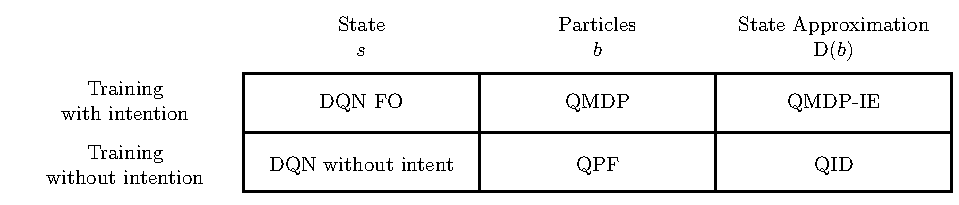
\includegraphics[width=0.85\textwidth]{figures/figures-algorithms.pdf}
        \caption{Table showing the difference between proposed algorithms. The first row are algorithms that have access to the true intention during training, while the algorithms on the second row do not. The columns show the input to the neural network, where the first column contains the baseline algorithms that use the noisy observation from the sensors either with or without the intention $i^j$. The second column contains algorithms using all $M$ particles as input and the final column uses an estimate of the intention.}
    \label{fig:algorithms}
\end{figure*}
This section describes the proposed approach to train an \gls{rl} agent in the belief space. 
In classical deep \gls{rl} methods for POMDPs, the learned value function processes a sequence of observations using recurrent neural networks~\cite{HausknechtS15drqn} or by concatenating a finite history of observations and feeding it to a simple feed forward neural network~\cite{Mnih2015}. In this approach, a state estimation algorithm is used instead to compute a belief state based on the sequence of past observation and action. The resulting distribution is then fed to a deep \gls{rl} agent. 
Instead of processing observations, our agent processes belief states. By learning in the belief space, our agent is more robust to state uncertainty and, contrary to the QMDP approach, it can compensate for some limitations of the state estimation module. 
This ability is key to learning intention aware policies for autonomously navigating intersections.

All six algorithms in this paper follow the same deep Q-learning structure, shown in \ref{alg:training_process}, with the added subtlety that the architecture of the value function, in step $10$ from \ref{alg:training_process}, varies in order to process belief states. 
The loss function in \ref{eq:dqn-loss} takes the form of a mean-squared error with a target corresponding to $r +  \gamma \max_{a^\prime}Q(s^\prime, a^\prime; \theta)$ and a prediction corresponding to $Q(s, a; \theta)$. 
Depending on the algorithm presented, the prediction will be performed in a different way.

To confirm the hypothesis that the intention state is necessary, two baseline \gls{dqn} algorithms are used. 

\textbf{DQN FO}: This algorithm is trained with full observability and has access to the true intention at training. As mentioned earlier, intention can not be measured directly, and therefore this algorithm is just used to show the best policy if the intention approximation is accurate. It also assumes perfect observability of the other state variables.

\textbf{DQN without intention}: Compared to the previous algorithm, this has access to the same states except the intention. By omitting the intention from the input state that is fed to the neural network, this baseline algorithm can be used to show the limit of a policy that does not have access to the intention.

\textbf{QMDP}: The first approach to use the belief state is the QMDP approach described in \ref{eq:qmdp}. 
The belief state is used at test time but the agent is trained in an environment with full observability in order to estimate $Q_{\text{MDP}}$. The prediction used in the loss function is $Q(s, a)$ and is learned from $(s, a, r, s')$ tuples.
The resulting policy can be sensitive to the performance of the state estimation algorithm used to generate the belief state $b$. 
To address this issue, we use the true state at training time so that the training procedure matches what the agent will experience at test time. 

\textbf{QPF (Particle Filter)}: With this algorithm, the agent is trained in an environment with partial observability and uses our proposed particle filter algorithm. 
The input to the agent is a set of $M$ particles. 
The loss function is minimized from $(b, a, r, b')$ experience samples and the Q-learning prediction is given by:
\begin{equation}
    Q(b, a; \theta) = \frac{1}{M} \sum_{m=1}^M Q(s^{[m]}, a; \theta).
\end{equation}
This operation is differentiable and allows training $Q(b, a)$ using deep Q-learning. 
One challenge with this approach is that the number of particles used to represent the belief can be very large in practice and cause the training to be unstable and very slow. It is challenging to update the individual Q-values by back propagating the loss function computed based on an aggregation of the values of many particles.

\textbf{QID (Intention Distribution)}: The agent is also trained in an environment with partial observability and the loss is minimized using $(b, a, r, b')$ samples. To simplify the training procedure compared to QPF, the probability distribution of the intention is used to compute the prediction:
\begin{equation}
    Q(b, a; \theta) = Q(\text{D}(b), a; \theta)
\end{equation}
where 

\begin{equation}
    \text{D}(b) = (p^\mathrm{ego}_\mathrm{goal},p^\mathrm{ego}_\mathrm{int}, v^\mathrm{ego}, t_\mathrm{stop}, \{\hat{p}^{j}_\mathrm{int}, \hat{v}^j, \tilde{i}^j\}_{j=1}^N),
    \label{eq:IE_b}
\end{equation}
and the probability distribution of the intention
\begin{equation}
    \tilde{i}^j = \sum_{m=1}^M w^{j,[m]} [\tilde{i}_\text{take} , \tilde{i}_\text{give}]^{j,[m]}
\end{equation}
is given by the particle filter, where $w^{j,[m]}$ is the weight of the particle $m$ and $[\tilde{i}_\text{take} , \tilde{i}_\text{give}]$ is the one-hot vector specifying intention. 
This operation does not affect the differentiability of the Q function that is trained using the same procedure as QPF. 
The advantage of this approach is that, at training time, the agent can experience changes in the estimated intention that would match what the state estimator would produce at test time.
As a consequence, the agent becomes more robust to the error in intention estimation.


\textbf{QMDP-IE (Intention Estimate)}: The last algorithm consists of training an agent on a fully observable MDP just like the QMDP approach. At test time, instead of averaging the Q-values of all the particle, a threshold $i_\text{threshold}$ is set on the intention distribution and then use it as the true intention state. 
Similar to \ref{eq:IE_b}, the particle filter is only used to generate the intention and is represented as a one-hot vector
\begin{align}
\hat{i}^j = & \begin{cases}
[0 \; 1] & \text{if } \tilde{i}^j_\text{give} > i_\text{threshold}\\
[1 \; 0] & \text{otherwise,}
\label{eq:IE_i}
\end{cases} 
\end{align}
where a high value on the threshold $i_\text{threshold}$ makes the agent more conservative. 


\section{Experiments}
\label{sec:experiments}
We present in this section the experiment setup in three steps. First, we describe how the simulator generates the different traffic scenarios. Second, the network architecture is defined. Third, we describe the details of the training procedure. 
%This section describes the experiment setup. We start by describing how the simulator generates the different traffic scenarios, then we define the network architecture and the training procedure.

\begin{algorithm}[!t]
    \caption{Training process}\label{alg:training_process}
    \begin{algorithmic}[1]
        \State Initialize $\theta$ randomly
        \State $\mathcal{D} \gets \emptyset$
        % \State $t \gets 0$
        \For{nr episodes}
            \State $o \gets $ initiate environment
            \State $b \gets $ \Call{InitializeBelief}{$o$}
            \While{episode not finished}
                \If{$e \sim \mathcal{U}(0,1) < \epsilon$}
                    \State $a \gets \mathrm{random\ action}$
                \Else
                    \State $Q(b, a) \gets $\Call{GetActionValues}{$b, \theta$}
                    \State $a \gets \argmax_{a} Q(b,a)$
                \EndIf
                \State $o^\prime, r \gets $ \Call{StepEnvironment}{$a$}
                \State $b^\prime \gets $ \Call{UpdateBelief}{$b$, $o^\prime$, $a$}
                   \State $\mathcal{D} \gets \mathcal{D} \cup \{(b, a, r, b^\prime)\}$
                   \State $M \gets $ sample from $\mathcal{D}$
                   \State update $\theta$ with SGD and loss $J(\theta)$ 
                % \State $t \gets t + 1$
            \EndWhile
        \EndFor
        % \Function{UpdateBelief}{$b_t, \theta$}
        % 
        % \EndFunction
    \end{algorithmic}
\end{algorithm}

% \begin{algorithm}[!t]
%     \caption{QMDP}\label{alg:QMDP}
%     \begin{algorithmic}[1]
%         \Function{GetQValues}{$b_t, \theta$}
%         % Q-values for all particles
%         % Take mean
%         % Return mean
%         \EndFunction
%     \end{algorithmic}
% \end{algorithm}

% \begin{algorithm}[!t]
%     \caption{QPF}\label{alg:QID}
%     \begin{algorithmic}[1]
%         \Function{GetQValues}{$b_t, \theta$}
%         % Get MLE of belief
%         % Get Q-value for belief
%         % Return mean
%         \EndFunction
%     \end{algorithmic}
% \end{algorithm}

% \begin{algorithm}[!t]
%     \caption{QID}\label{alg:QID}
%     \begin{algorithmic}[1]
%         \Function{GetQValues}{$b_t, \theta$}
%         % Get MLE of belief
%         % Get Q-value for MLE belief
%         % Return Q-value
%         \EndFunction
%     \end{algorithmic}
% \end{algorithm}

\subsection{Simulator setup}
\label{sec:simulation_setup}

\begin{figure}[!t]
    \centering
        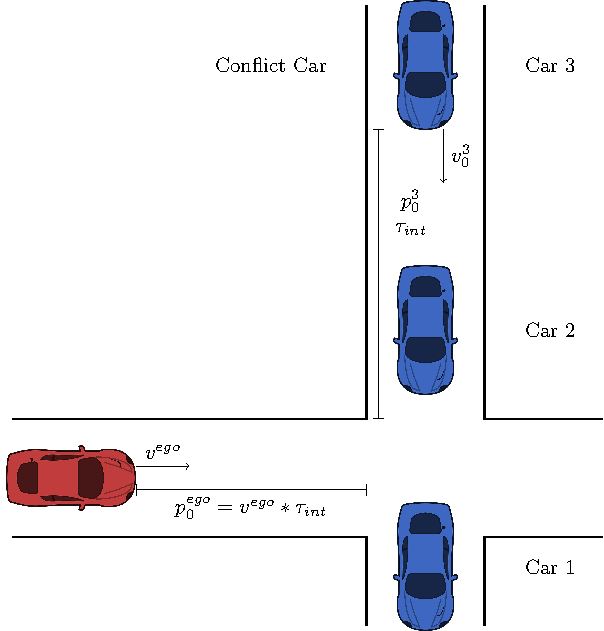
\includegraphics[width=0.7\columnwidth]{figures/figures-conflict_car.pdf}
        \caption{Initial state with three other cars and ego car initial position is set to have the same time to intersection as the conflict car, in this case car 3.}
    \label{fig:conflict_car}
\end{figure}


At the start of each episode, up to $N$ vehicles are spawned with initial positions $p^j_0$ distributed along the intersecting lane, a starting velocity $v^0$, and a desired velocity $v^j_\mathrm{desired}$. Each vehicle is spawned with a deterministic policy that represents their intention, which can be either take way or give way as described in \ref{sec:action}. The ego vehicle is spawned last with an initial speed $v^\mathrm{ego}$ and desired speed $v^\mathrm{ego}_\mathrm{desired}$. The starting position of ego is then set based on the time to intersection $\tau_{int}$ of one of the other vehicles. This other car is referred to as conflict car. The initial position of the ego becomes: 
\begin{equation}
    p^\mathrm{ego}_{0} = v^\mathrm{ego} \frac{p^{c}_{0}}{v^{c}_{0}},
\end{equation}
where $c$ is the index of the conflict car. This initialization increases the probability that the ego will conflict with at least one other car as shown in~\ref{fig:conflict_car}. 

% \subsubsection{Run time}
The decision time between decisions steps are $\mathrm{d}t_{\text{decision}}$. For every decision step, the simulator updates the objects states four times with a simulation time $\mathrm{d}t_{\text{sampling}}$, checking for terminal states at each update. 
The simulator keeps track of the true state of all objects. An observation model is used to add noise to each observation, following \ref{eq:noise_pos,eq:noise_vel}. The update function updates the true state $s_t$. 
Every time a vehicle in the perpendicular lane crosses the intersection, they are re-spawned at the start of the lane at a random time with new initial states and intention.

% \subsubsection{terminal state}
The possible terminal states are the following:
\begin{enumerate*}[label=(\roman*)]
  \item Goal, ego vehicle reaching the goal.
  \item Collision, ego collides with one of the other vehicles.
  \item Safe stop, if the ego vehicle has been standing still for more than $T_\mathrm{stop}$ seconds and no other car is standing still. 
  \item Deadlock, if another vehicle standing still at the intersection yielding for the ego vehicle and while the ego vehicle has also been standing still for more than $T_\mathrm{stop}$ seconds. 
  \item Timeout, if the total simulation time exceeds $T_{lim}$. 
\end{enumerate*}
Each of these terminal states, except for the simulation timeout, has a corresponding reward, described in \ref{sec:reward}. The terminal state referred to as collision in this paper may sound drastic, but could also be interpreted as intervention by a collision avoidance system.

\begin{table}[!bt]
	% increase table row spacing, adjust to taste
	\renewcommand{\arraystretch}{1.2}
	\caption{Hyperparameters of Simulator}
	\label{tab:hyperparameters}
	\centering
	\begin{tabular}{l l r}
		\toprule
		%Parameter & Value\\
		sampling time [\si{\second}], & $\mathrm{d}t_\mathrm{sampling}$ & $0.5$\\
		decision time [\si{\second}], & $\mathrm{d}t_\mathrm{decision}$ & $2$\\
		initial speed [\si{\meter\per\second}], & $v^o_0 $ & $2-7$\\
		initial acceleration [\si{\meter\per\second\squared}], & $a^o_0 $ & $0$\\
		desired speed [\si{\meter\per\second}], & $v_\mathrm{desired}^o$ & $2-7$\\
		time gap [\si{\second}], & $T_\mathrm{gap}$ & $1.5$\\
		Stop time limit [\si{\second}], & $T_\mathrm{stop}$ & $10$\\
		Timeout time [\si{\second}], & $T_\mathrm{lim}$ & $120$\\
		ego spawn speed [\si{\meter\per\second}], & $v^\mathrm{ego}$ & $5$\\
		ego desired speed [\si{\meter\per\second}], & $v^\mathrm{ego}_\mathrm{desired}$ & $5$\\
		noise position [\si{\meter}], & $\sigma_\mathrm{p}$ & $2$\\ 
		noise velocity [\si{\meter\per\second}], & $\sigma_\mathrm{v}$ & $1$\\ 
		max observed vehicles, & $N$ & $4$\\ 

        \midrule
        IDM max acceleration [\si{\meter\per\second\squared}], & $\alpha^{\mathrm{max}} $ & $0.73$\\
        IDM deceleration [\si{\meter\per\second\squared}], & $\alpha_b $ & $0.5 - 4.0$\\
        IDM acceleration exponent, & $\delta$ & $4$\\
        IDM minimum distance [\si{\meter}], & $s_0$ & $2$\\
		\midrule
		
		number of particles & $n_b$ & 100\\
		acceleration noise [\si{\meter\per\second\squared}] & $\sigma_a$ & 0.1 \\
		intention switch probability & $p_i$ & 5 \\
		intention probability threshold & $i_\text{threshold}$ & 0.8 \\
		\midrule
		
		Batch size & B & $128$ \\
		Learning rate & lr & $0.0001$ \\
		Discount factor & $\gamma$ & $0.95$\\
		Replay memory size & $M_\mathrm{replay}$ & $20{,}000$\\
		Target network update frequency & $N_\mathrm{update}$ & $1{,}000$\\

% 		Initial exploration constant, $\epsilon_\mathrm{start}$  & $1$\\
% 		Final exploration constant, $\epsilon_\mathrm{end}$ & $0.05$\\
% 		Final exploration iteration, $N_{\epsilon\mathrm{{\mathrm -}end}}$ & $1{,}000{,}000$\\

		\bottomrule
	\end{tabular}
\end{table}


\subsection{Neural network architecture}
 The neural network architecture that is used in this study is shown in~\ref{fig:network}. A previous study~\cite{Hoel2018} introduced applying a convolutional operator to the states that describe the surrounding vehicles. With this structure, the states that describe each surrounding vehicle are passed through the same weights. The size and stride of the convolutional layer is set to $(4, 1)$, where four equals the number of states that describe each vehicle and one means that the different particles are handled individually. The convolutional layer uses \num{32} filters with a $\tanh$ activation function. To speed up learning, the index $j$ are ordered by distance $p^j_\mathrm{int}$ starting from the vehicle closest to the intersection and a default state used for cars that do not exist. 

The ego vehicle states are passed through a fully connected layer of size $32$ before being concatenated with the output of the convolutional layer. The output of the concatenated layer is then passed through two fully connected layers of size $32$ and finally a fully connected layer of size two gives the $Q$-values. These values are then merged according to one of the algorithms in \ref{sec:belief_state_rl} to form a combined estimate of the $Q$-values. The belief dimension of the neural network represents the number of particles $n_b$ that are passed through the network. This number varies depending on which algorithm that is used as discussed in \ref{sec:belief_state_rl}.


\begin{figure}[!t]
    \centering
        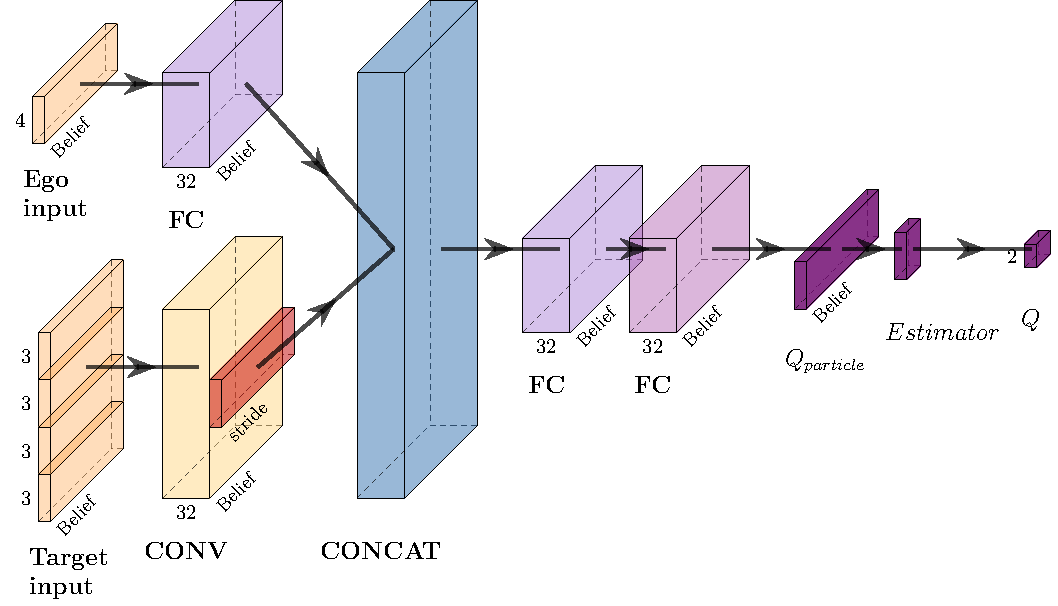
\includegraphics[width=0.9\columnwidth]{figures/belief.pdf}
        \caption{Network architecture, where ego input represents the input features for the ego vehicle, $p^\mathrm{ego}_\mathrm{goal},p^\mathrm{ego}_\mathrm{int}, v^\mathrm{ego}, t_\mathrm{stop}$, and Target input $\{p^{j}_\mathrm{int}, v^j, i^j\}_{j=1}^N$ for the the target vehicle $j$. The layers consists of one convolution (Conv) and a total of three fully connected (FC), where the depth of the layers represents the belief size.}
    \label{fig:network}
\end{figure}

\subsection{Training procedure}
\label{sec:training_procedure}
Each network was trained for \num{200000} episodes. The loss function of Double DQN is applied, which modifies the maximization operation of \ref{eq:dqn-loss} to $\gamma Q(s',\argmax_{a'} Q(s',a';\theta_i);\theta_i^-)$~\cite{Hasselt2016}. 
Stochastic gradient decent is used to update the weights~\cite{Kingma2014}. The hyper parameters of the training process are shown in \ref{tab:hyperparameters}, and the values were selected by an informal search due to the computational complexity. 

If the current policy of the agent do not reach a terminal state before the simulation timeout time $T_\mathrm{lim}$, an episode in the real world could continue forever. Therefore, when the simulation reaches the timeout state, the last experience of such an episode is not added to the replay memory. This trick prevents the agent from learning that an episode can end due to a timeout, because the terminating state is not part of the \gls{mdp}~\cite{Hoel2018}.

\section{Results / Results and discussion}
\label{sec:results}
This section presents the evaluation metrics and results from the experiments, presented in \ref{tab:results_summary}. Although the agents are train and evaluated on scenarios with different number of other cars. Because the scenario with four other cars is the hardest to cross without colliding, it is used to compare the performance of the different agents.

Each agent is evaluated on \num{1000} episodes. The random seeds are based on the episode number, which generates the same values for the random parameters, defined in \ref{tab:hyperparameters}, for each test scenarios when evaluating different agents.
The metrics of interests are the average time it takes for the agent to either reach the success state and how often each terminal state is reached. A success state refers to either reaching the goal or a safe stop, from \ref{sec:reward}, where both are considered good outcomes. For the purpose of this paper, it is more important to first find an agent with no collisions and no deadlocks, and then optimize for the time it takes to reach the goal. 

\begin{figure}[!t]
    \centering
        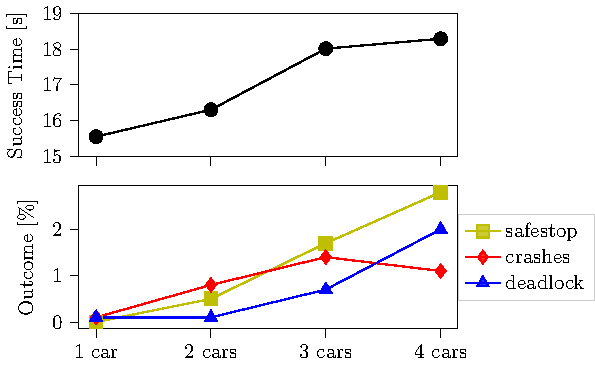
\includegraphics[width=0.99\columnwidth]{figures/figures-1-4cars.pdf}
        \caption{Performance results for DQN without intention algorithm, showing the increasing difficulty for scenarios with different number of cars in the environment.}
    \label{fig:number_cars}
\end{figure}


\begin{table}
\caption{Result summary for scenario $N=4$ cars}
\label{tab:results_summary}
\begin{tabularx}{\columnwidth}{@{}l*{10}{c}c@{}}
\toprule
Experiments     & Goal reached & Safe stop & Collision & Deadlock & Success time & Training time\\ 
\midrule
DQN FO & $94.20$ & $5.60$ & $\textbf{0.00}$ & $0.20$ & $16.93$ & $1\si{\day}7\si{\hour}$ \\ 
DQN w/o intent & $94.10$ & $2.80$ & $1.10$ & $2.00$ & $18.29$ & $1\si{\day}7\si{\hour}$ \\ 
QMDP & $93.70$ & $5.60$ & $\textbf{0.10}$ & $0.60$ & $19.95$ & $1\si{\day}7\si{\hour}$ \\ 
QMDP-IE & $94.70$ & $4.80$ & $\textbf{0.00}$ & $0.50$ & $17.60$ & $1\si{\day}7\si{\hour}$ \\  
QPF & $84.70$ & $8.90$ & $3.60$ & $2.80$ & $20.16$ & $2\si{\day}17\si{\hour}$ \\ 
QID & $\textbf{97.00}$ & $0.90$ & $2.00$ & $0.10$ & $\textbf{16.90}$ & $2\si{\day}10\si{\hour}$ \\ 
\bottomrule
\end{tabularx}
\end{table}


\subsection{Baseline DQN results}
The agent trained with full observability, DQN FO, shows how well an agent could perform if it had access to the true intention of other drivers. From \ref{tab:results_summary}, the DQN FO agent has \SI{94.2}{\percent} goals reached, \SI{5.6}{\percent} safe stops, \SI{0}{\percent} collisions, \SI{.2}{\percent} deadlocks, and an average success time of \SI{16.93}{\second}. 
While DQN without intention has \SI{94.1}{\percent} goal reached, \SI{2.8}{\percent} safe stops, \SI{1.1}{\percent} collisions, \SI{2.0}{\percent} deadlocks, and reached the goal slower with an average time of \SI{18.29}{\second}.
The difference in collision rates confirms our hypothesis that a agent trained with an intention state is better than one without. DQN with intention was both faster to reach the goal and could do it with zero collisions in the evaluation space.
All agents are trained with a variable number of other vehicles. \ref{fig:number_cars} shows the performance difference with increasing number of vehicles. In scenarios with only one other vehicle, the agent trained using DQN without intention found a policy that could avoid collisions. However, increasing the number of other vehicles makes the problem harder to solve, which results in an increasing number of collisions and a longer success time. 


\subsection{QMDP and QMDP-IE results}
\begin{figure}[!t]
    \centering
        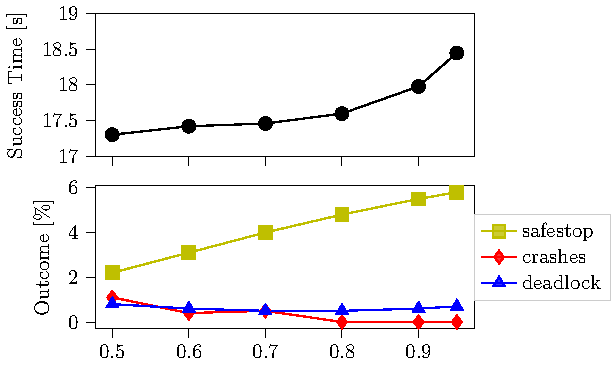
\includegraphics[width=0.99\columnwidth]{figures/figures-intention-t.pdf}
        \caption{QMDP-IE performance (aggressiveness) for different $i_\text{threshold}$ values. Increasing $i_\text{threshold}$ lowers the collision rate while at the same time increases the safe Stop rate and the time it takes to reach a success state.}
    \label{fig:intent_threshold}
\end{figure}

QMDP and QMDP-IE are both approximation algorithms that use the network trained on DQN FO. 
Both have similar outcome performance, QMDP reached the goal \SI{93.7}{\percent}, safe stopped \SI{5.6}{\percent}, collided only \SI{0.1}{\percent}, and got stuck in deadlock \SI{0.6}{\percent} with an average success time of \SI{19.95}{\second}. for QMDP-IE, the performance for different threshold values of $i_\text{threshold}$ are shown in~\ref{fig:intent_threshold}. 
The lowest threshold $i_\text{threshold}=0.5$ is equivalent to just taking the most likely estimation of the intention and it has the most aggressive behaviour with the lowest percentage of safe stops, highest collisions and the fastest time to reach the goal. When the threshold increases, so does the safe stop rate and the time it takes to reach the goal, while the collision rate decreases and deadlock rates stay about the same. 
An agent with $i_\text{threshold}=0.8$ was the lowest threshold that achieve zero collisions during testing and is therefore chosen as the threshold value when compared to the other agents in \ref{tab:results_summary}. 
With $i_\text{threshold}=0.8$, QMDP-IE has \SI{43.7}{\percent} goal reached, \SI{4.8}{\percent} safe stops, \SI{0.0}{\percent} collisions, \SI{0.5}{\percent} deadlocks, and with an average success time of \SI{17.60}{\second}
Compared to DQN without intention, that has a success time of \SI{18.29}{\second}, QMDP is more conservative with a slower success time of \SI{19.95}{\second}, while the QMDP-IE is faster with \SI{16.90}{\second}. 


The proposed particle filter performs well at estimating the probability distribution of the intention. However, it relies on an accurate prediction model. %The accuracy was very correlated with the noise of the probability distribution. 
It is possible to improve the estimate by increasing the number of particles at the expense of additional computation.

\subsection{QPF and QID results}
The algorithms that do not have access to the intention during training, QPF and QID, reach the goal much less frequently. QPF has the lowest goal reached rate at \SI{84.7}{\percent}, \SI{8.9}{\percent} safe stop, the highest collision rate at \SI{3.6}{\percent}, \SI{2.8}{\percent} deadlocks, and the highest average success time of \SI{20.16}{\second}. QID learned the most aggressive policy, with \SI{97.0}{\percent} goal reached, \SI{0.7}{\percent} safe stop, \SI{2.0}{\percent} collision, \SI{0.1}{\percent} deadlock and the fastest average success time of \SI{16.90}{\second}, which is equal to the \gls{dqn} baseline algorithm. As mentioned in the beginning of the section, the a slightly higher collision rate of \SI{2.0}{\percent} classifies this performance as poor compared to QMDP and QMDP-IE, but it is much better than QPF on all evaluation metrics. 
The higher collision rate could be because of the larger state space, which could create some instability during training. The particle filter was also not fully optimized, because we wanted to investigate if the approximation of the \gls{dqn} could compensate for the noisy states of the particles. 
Finally, it should be noted that it required almost two and a half days to train QPF and QID, which is almost twice as much time required to train the fully observable network. 


\subsection{Discussion}

\label{sec:discussion}
\textit{Is it better to train on the full distribution of the belief or use an estimation of the intention?} When comparing QPF and QID to their baselines, it is observed that both algorithms that were trained on the ground truth outperform the algorithms that were trained using the belief state or even just an estimate of the belief distribution. Both QMDP and QMDP-IE had zero collisions in the evaluation space just like DQN FO, while QMDP-IE had a slightly faster policy. 


We used a particle filter to create the belief state and filter the noisy observations, hoping the flexibility of the neural network would be able to compensate for some of the inaccuracy of the belief in the same way it can approximate the noise. The higher collision rate for the QPF compared to QMDP shows that training on the full set of beliefs can make finding a good policy difficult. 


\ref{fig:intent_threshold} shows that the aggressiveness of the policy from QMDP-IE is correlated with $i_\text{threshold}$ and by choosing a relatively high value at $0.8$ the policy could achieve zero collisions in the evaluation space and in this case could to some extent compensate for the loosely optimized particle filter. The ability to adjust the aggressiveness of the policy by changing $i_\text{threshold}$ is also a strength of QMDP-IE compared to our previous black box methods that use an \gls{lstm} to estimate the latent state~\cite{Tram2018}. %For QMDP and QMDP-IE, it is not unreasonable to assume that the true intention of other drivers is accessible during training. These intentions can be labeled after the fact, by looking at if the driver ended up crossing the intersection or stopping before it. 

\section{Conclusion}
\label{sec:conclusion}
In this paper, we use a particle filter implementation to maintain a belief state to train an \gls{rl} agent using a \gls{dqn}. 
A set of four different algorithms are evaluated with the aim to find the safest and fastest policy that can drive through an intersection crossing traffic participants that has a latent intentions state. 
Two algorithms, QMDP and QMDP-IE, use a network trained with access to the true intention of the other vehicles but was evaluated with an estimate of their intention. Both algorithms could find a policy with zero collisions in the evaluation space, while QMDP-IE lead to the most efficient policy.
The other two algorithms, QPF and QID, were trained without access to the true intention state and could not achieve a policy without collisions. 
The QID agent had the fastest average time to reach the goal, but resulted in collision more often than the baseline \gls{dqn} agent. As for the QPF agent, training on the entire belief state as input yielded the worst performance of all evaluated algorithms. It seems reasonable that the results can be improved by using a network structure that can better learn the latent state. One such candidate is Deep Variational Reinforcement Learning proposed by \citet{Igl2018}. 